%
% Project proposal
% Guidelines can be found at: http://courses.cse.tamu.edu/caverlee/csce470/project.html
% 
\documentclass{article}
\renewcommand{\contentsname}{Table of Contents}
\newcommand{\PaperTitle}{Executive Summary}
\usepackage{hyperref}
\usepackage{fullpage}
\usepackage{graphicx}
\usepackage{wrapfig}

%\hypersetup{colorlinks=false}

\begin{document}

%
% Title Page
\newcommand{\HRule}{\rule{\linewidth}{0.5mm}}
%
% Title Page
%
\begin{titlepage}
  \begin{center}
  % Title
  \textsc{\Large FootTraffic}\\[0.5cm]
  \HRule \\[0.4cm]
  {\huge \bfseries \PaperTitle}\\[0.2cm]
  \HRule \\[1cm]
  
  \large{Department of Computer Science \& Engineering} \\
  \large{Texas A\&M University} \\[1cm]

  % Authors and emails
  \begin{minipage}{0.4\textwidth}
    \begin{flushleft} \large
    \emph{Authors:}\\
    William \textsc{Chen} \\
    Eric \textsc{Wood}
    \end{flushleft}
  \end{minipage}
  \begin{minipage}{0.4\textwidth}
    \begin{flushright} \large
    \emph{Emails:} \\
    wchen16@cse.tamu.edu\\
    ebw0178@cse.tamu.edu
    \end{flushright}
  \end{minipage}
  \\[1cm]
  \large{\today}
  \vfill
  
  % Bottom of the page
  \end{center}
\end{titlepage}


%
% Document
% Motivation and Related Works
\section{Motivation and Related Works}
We are seeing an increasing amount of location sharing from social services Foursquare, Facebook, Google Latitude, etc.,
and we want to harness these traffic to recommend venues to users based on the traffic patterns. Most location-based
search engines today rank results based on proximity, user rating, category, and popularity. We want to add another 
dimension to location-based searches, and that is ranking based on observed traffic similarities.
This ``\textit{temporal dynamics embedded in the checkins} from location sharing services''
\footnote{``\href{http://faculty.cs.tamu.edu/caverlee/pubs/cheng11cikm.pdf}{Toward Traffic-Driven Location-Based Web Search}''
  by Zhiyuan Cheng, James Caverlee, Krishna Y. Kamath, and Kyumin Lee; CIKM 2011},
approach is introduced by a research paper authored by Zhiyuan Cheng, James Caverlee, Krishna Y. Kamath,
and Kyumin Lee, and the foundation of FootTraffic search engine will be based on the ideas from the paper
\footnote{A copy of the paper can be found at: \url{http://faculty.cs.tamu.edu/caverlee/pubs/cheng11cikm.pdf}}
aforementioned.

\section{Our Approach}
\begin{wrapfigure}{r}{6cm}
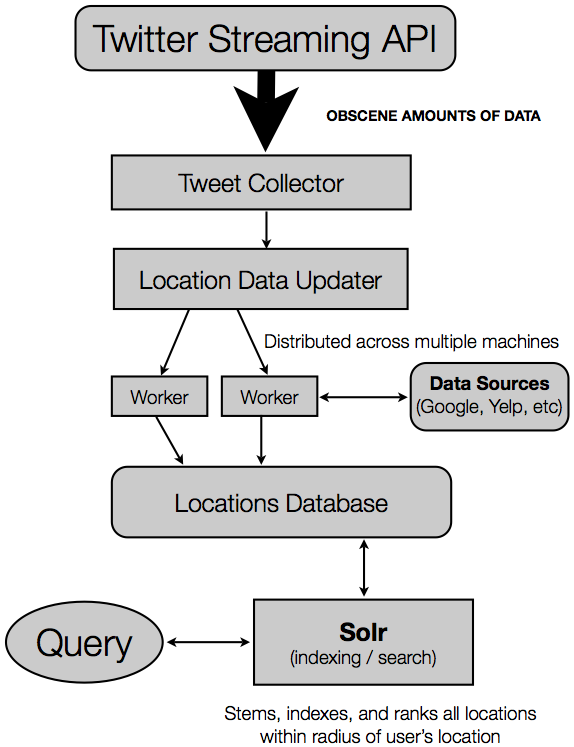
\includegraphics[width=6cm]{flowchart.png}
\caption{Workflow}
\end{wrapfigure}
We have put in a lot of thought into creating efficient and optimized ways of gathering, storing, and serving data. The final solution
we came up with is outlined in the flowchart shown to the right. In the backend, we have scripts, an Apache server with Phusion Passenger
to run Ruby on Rails, a \href{http://lucene.apache.org/solr/}{Solr} instance, and a Postgres database server. In the frontend, we used
a couple Javascript libraries and APIs, such as JQuery, Google Fonts, Google Maps, flot, to handle events and transitions. 
\\ \\
We have two scripts that are run continuously and concurrently. One is responsible for keeping a connection open with Twitter's realtime
search API, filtering for FourSquare tweets, and inserting an entry to a database table (Checkins). The other is responsible for processing
entries in the Checkins table, then requesting information from Yelp and Google. If the venue exists already in our database, no additional
API calls are made, and the traffic data is updated accordingly. 
\\ \\
Lorem ipsum dolor sit aet, consectetur adipiscing elit. Maecenas in quam risus. Maecenas orci neque, vulputate in ultrices sagittis, accumsan vel lectus. Curabitur quis feugiat magna. Quisque porttitor tempor leo, nec gravida sem vestibulum quis. Nullam viverra nunc ut felis volutpat ac ullamcorper velit dictum. Aenean bibendum neque non orci porta venenatis. Pellentesque sed tellus arcu, et consequat elit. Ut lorem metus, suscipit ut tincidunt et, fermentum quis lorem. Aenean quis diam vitae sem gravida pretium.

\subsection{Ranking}
\subsection{Challenges}

\section{Evaluation}

\end{document}
